\begin{frame}
    \frametitle{Présentation générale}
  	\begin{block}{Historique}
  	\begin{itemize}
  		\item Japonais au XVIIIème siècle
  		\item Richard Dow (graphique) puis Nison (chandelier), Bollinger
	\end{itemize}
	
	\end{block}
	\pause
	\begin{block}{Définition}
		\begin{itemize}
			\item John Murphy : " L’analyse technique est l’étude de l’évolution d’un marché, principalement sur la base de graphiques, dans le but de prévoir les futures tendances ".
		\end{itemize}
	\end{block}
\end{frame}

\begin{frame}
    \frametitle{Tendances}
  	\begin{block}{Présentation}
  		Les lignes de tendances sont la loi de base de l’analyse technique :
  		\begin{itemize}
  			\item \textbf{La résistance} rejoint les points hauts de la courbe de valeur du cours.
  			\item \textbf{Le support} de même avec les points les plus bas
  		\end{itemize}
  		\center
  	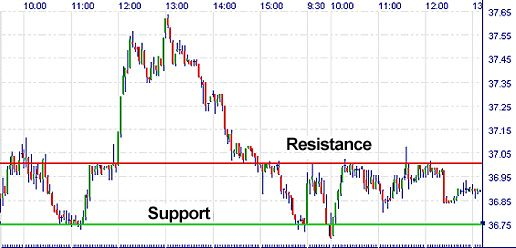
\includegraphics[scale=0.3]{images/supportresistance.jpg}

	\end{block}
\end{frame}

\begin{frame}
    \frametitle{Chandelier}
    	\begin{block}{Définition}
  		Les chandeliers sont des indicateurs graphiques permettant de représenter la variation d'un cours sur la journée :
  		\begin{itemize}
  			\item \textbf{La chandelier blanc} signifie une hausse du cours.
  			\item \textbf{La chandelier noir} signifie une baisse du cours.
  		\end{itemize}
  		\center
  	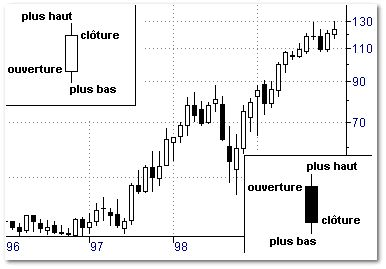
\includegraphics[scale=0.3]{images/chandelier.png}
	\end{block}

\end{frame}

\begin{frame}
    \frametitle{Exemples de figures significatives}
       	\begin{columns}
		\begin{column}{3.5cm}
		  \begin{figure}
		      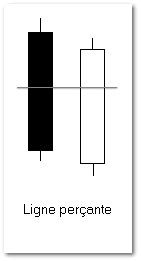
\includegraphics[scale=0.45]{images/chandelier1.png}
		      \caption{Ligne Perçante}		   
		  \end{figure}
		\end{column}
		\begin{column}{3.5cm}
		  \begin{figure}
		      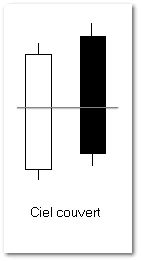
\includegraphics[scale=0.45]{images/chandelier2.png}
		      \caption{Ciel Ouvert}	   
		  \end{figure}
		\end{column}
		\begin{column}{3.5cm}
		  \begin{figure}
		      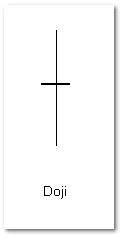
\includegraphics[scale=0.49]{images/chandelier9.png}
		      \caption{Doji}	   
		  \end{figure}
		\end{column}		
	\end{columns}

\end{frame}

\begin{frame}
    \frametitle{Moyenne mobile}
      	\begin{block}{Définition}
  		\begin{itemize}
  			\item $MM$ : moyenne des cours sur une période donnée.
   			\item $MME = fermeture du jour * 0.09 + MM de la veille * 0.91$. 
		\end{itemize}
	\end{block}
	\begin{figure}
	    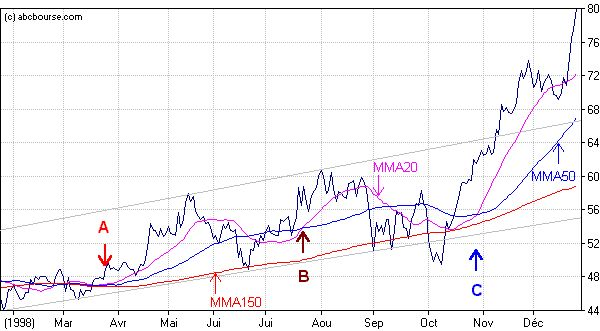
\includegraphics[scale=0.3]{images/moyennemobile.png}   
	\end{figure}
\end{frame}


\begin{frame}
    \frametitle{Bollinger}
    \begin{columns}
      \begin{column}{5cm}
	  \begin{block}{Calcul des bandes}
		\begin{itemize}
		\item Moyenne mobile sur une période de n = 20.
		\item Bande supérieure : $MMn + x \times ecartType$
		\item Bande inférieure : $MMn - x \times ecartType$
		\item $ecartType= \sqrt{\sum{\frac{(cloture-MMn)^2}{n}}}$
		\end{itemize}
	  \end{block}
      \end{column}
    \begin{column}{5cm}
	\begin{figure}
	      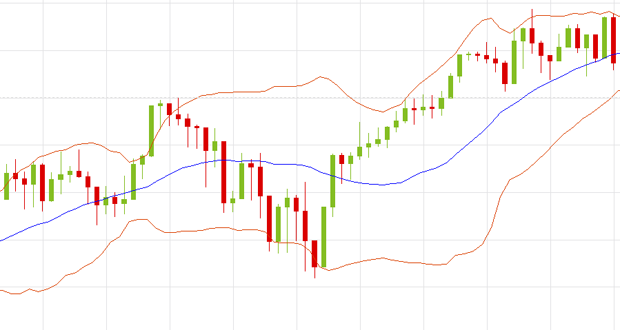
\includegraphics[scale=0.25]{images/bollinger.png}
	      \caption{Bandes de Bollinger}
	  \end{figure}   
	\end{column}
    \end{columns}
\end{frame}

\begin{frame}
    \frametitle{Bollinger}
    \begin{columns}
      \begin{column}{5cm}
	  \begin{block}{Interprétation}
		\begin{itemize}
		\item Tendance clairement définie, regarder quand le cours intercepte la bande.
		\item Si pas de tendance, regarder quand on croise la bande.
		\item Etranglement : attention !
		\end{itemize}
	  \end{block}
      \end{column}
    \begin{column}{5cm}
	\begin{figure}
	      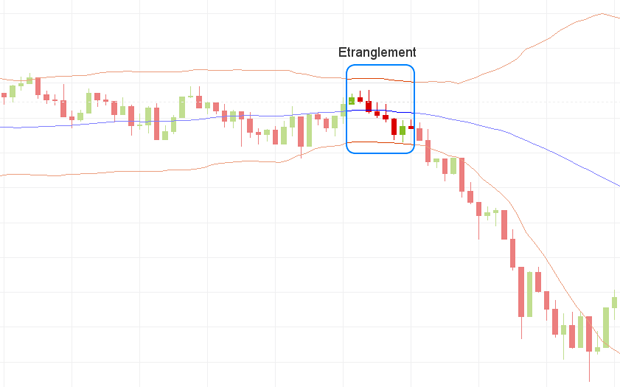
\includegraphics[scale=0.25]{images/bollingerEtranglement.png}
	      \caption{Exemple d'étranglement.}
	  \end{figure}   
	\end{column}
    \end{columns}
\end{frame}

\begin{frame}
    \frametitle{Volume}
    \begin{columns}
	\begin{column}{4cm}
	  \begin{block}{Définition}
		  \begin{itemize}
			  \item Nombre de titres échangés sur la journée (ou par prix).
			  \item Combiné à d'autres indicateurs.
		  \end{itemize}
	  \end{block}
	\end{column}
	\begin{column}{6cm}
	  \begin{figure}
	      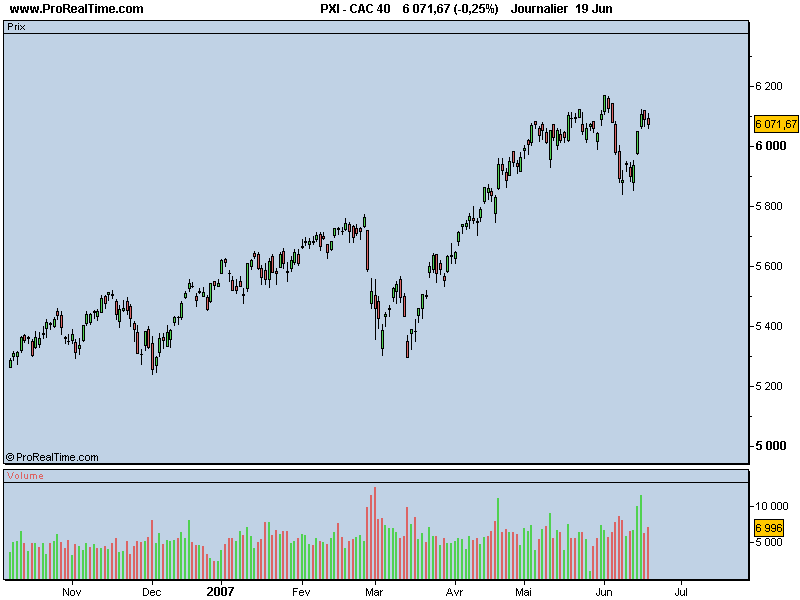
\includegraphics[scale=0.22]{images/volumeBarre.png}   
	  \end{figure}   
	\end{column}
    \end{columns}
\end{frame}
